
% CHAPTER:  1
% (Note: cannot have a footnote on a word within the \chapter{} construct, it does not work)
\chapter{UKIDSS}
\label{chap:ukidss}

\section{Intro: wavelength dependence on morphology: optical and IR}

Historically, visual morphological classification of galaxies has been conducted on optical images. Blue B-band images were the primary source dating back to Hubble's classic tuning-fork classification scheme \citep{Hubble1926} and in the subsequent modifications by \citet{Sandage1961} and \citet{DeVaucouleurs1963}. The more recent and larger morphological catalogs also derive their classifications from rest-frame optical images, either single-band (\citet{RC31991} (B-band), \citet{Scarlata2007} (ACS I-F814W), \citet{Fukugita2007} and \citet{Nair2010} (SDSS g-band)) or color-composite (\citet{Lintott2008}, \citet{Willett2013} (SDSS-gri)). 

In the optical regime, the flux is dominated by young, hot stars; this results in an emphasis of spiral structure in the images, but they tend to have patchy appearances due to the abundance of star-formation regions in the arms. Optical images also are impacted by extinction due to dust, which can obscure features that tend to be composed of older stellar components (such as bars and bulges). Longer wavelenths are free of these effects, making them ideal for revealing the underlying ``stellar backbone'' of galaxies.

It is possible, then, to consider two morphologically distinct components of a galaxy: a gas-dominated Population I disk, and a star-dominated Population II disk. The Population I disk is most easily seen in the optical, revealing HII regions, cold HI gas, and emission from young OB stars; these regions will tend to highlight flocculance in spiral structure. The Population II disk, on the other hand, traces the underlying mass distribution; consisting of the old, cooler stellar population, it is more easily seen at longer wavelengths. \citet{Block1999} even suggests that two separate classifications schemes should be required for all galaxies; one for the Population I disk, which can be probed in optical and ultraviolet images, and a Population II disk, for which longer wavelength images, free of dust extinction, would be required. 

The extent to which the morphologies of the younger and older stellar populations are decoupled, however, is not yet clear. Early studies which directly compared optical and near-IR images found very significant differences between the two morphologies \citep{Hackwell1983,Thronson1989,Block1991,Block1994}. \citet{Block1999} goes as far as to sugget that there is no correlation between the two, and that the optically-definied Hubble tuning fork ``does not constrain the morphology of the old steallar Population II disks.'' However, all of the aforementioned studies only compared morphologies of either a single galaxy, or at most a handful, so these conclusions cannot be applied generally.

The advent of larger surveys incorporating near and mid-IR detectors enabled morphological comparisons between the two wavelength regimes on a much grander scale than had previously been achieved. New results contradicted those of the previous case-studies: in general, IR morphology was found to be well-correlated with optical morphology in larger samples of galaxies. \citet{Eskridge2002} compared near-IR H-band (1.65$\mu$m) Hubble-type classifications to B-band in a sample of 205 nearby spiral galaxies from the Ohio State University Bright Spiral Galaxy Survey (OSUBSGS). Applying deVaucouler's classification system, they found an overall good correlation between the two morphologies, but on average galaxies from Sa through Scd appeared one T type earlier in the H band than in the B band. In the IR images the bulge tended to appear more prominent and the spiral arms less knotty, which resulted in the slightly earlier classifications. For the earliest (optically S0/a and Sa) and latest-type galaxies (optically Scd through Sm), no difference in morphologies was found. This is an expected result for the earlier-types, since these have little ongoing star formation and very little dust, so it is expected that both optical and IR morphologies are dominated by old stars. This result is less intuitive for the later-type galaxies, as these are dominated by ongoing star formation. However, these galaxies are defined as having very weak or nonexistant bulges and poorly defined spiral structure. Since the main driver in the differences in morphology across wavebands was found in the intermediate spirals to be the relative prevalance of a bulge and difference in contrast and appearance of spiral arms, galaxies lacking these features should not, in fact, be expected to look different in the IR than the optical. 
 
\citet{Buta2010} obtained similar results comparing optical and mid-IR (3.6 $\mu$m) images from the \textit{Spitzer} Survey of Stellar Structure in Galaxies ($\rm S^4G$, \citet{Sheth2010}) in a large sample of 2,331 spiral galaxies. Like \citet{Eskridge2002}, the optical and IR classifications were very well correlated, with the most significant differences occuring for S0/a to Sc galaxies, where the 3.6 $\mu$m were on average slightly earlier than the B-band classifications.

%Bars! 
%invisible in optical, visible in IR examples
Infrared imaging is also often used in place of (or in addition to) optical to indentify stellar bars (e.g. \citet{Mulchaey1997,Knapen2000,Block2004,Sheth2008}). Like bulges, bars are primarily composed of old, red stars, and therefore better traced by longer wavelengths. In fact, it is not uncommon for an infrared bar to be completely invisible in the optical. Notable examples include NGC 1566 \citep{Hackwell1983}, NGC 1068 \citep{Thronson1989,Scoville1988}, NGC 309 \citep{Block1991}, NGC 4736 \citep{Block1994}, and NGC 4303 (Figure 1, \citet{Sheth2003}). This trend is not only limited to case-studies; for example, in a larger sample of 29 galaxies classified as unbarred in the optical, \emph{50\%} of these were found to be barred in the near-IR images \citep{Mulchaey1997}.

%bigger: bar fraction
The fraction of spiral galaxies which exhibit bars (defined as the bar fraction) has been measured extensively in optical images, and typically falls near 50\% when bars of all strengths are considered \citep{Masters2010}(should probably cite more). Since it is much more common to find an infrared bar in an optically unbarred galaxy than the reverse, it is expected that the bar fraction in the infrared will, in general, be higher than what has been measured in the optical. Some studies find a substantial increase: \citet{Seigar1998} for example spectulate that ``bars may always be present in disks at some level'', based on finding a bar fraction of 90\% when using infrared images (as compared to their optical measurement of 68\%). Although their sample consisted of only 45 galaxies total, they claim this measurement should represent the general population of spirals, because their selection was not biased towards barred galaxies. Other studies report similar increases in bar fraction in the infrared, albeit not quite as large. \citet{Knapen2000} in a similar sample size of ~50 galaxies find a bar fraction in the infrared of ~70\%, a strong increase from the optical 50\%. \citet{Eskridge2000} in sample of 186 galaxies measure a bar fraction of 72\% in the infrared which is \emph{double} that of their optical measurement. While these studies report significant increases in bar fraction as a function of wavelength, they do dispute the claim by \citet{Seigar1998}, emphasizing that at least 30\% of galaxies in their sample are truly unbarred across all wavelengths.

%same bar fraction
Other more recent studies find larger bar fractions in the infrared, not significantly so. \citet{Whyte2002} measure an increase from 72\% to 79\% in a sample of 72 galaxies, while \citet{Sheth2008} reports 60\% for both wavelengths. \citet{MenendezDelmestre2007} also found a slight increase from 63\% to 67\% in a sample of 151 galaxies, noting that although bars tended to appear stronger in the near-IR, on average they were not so weak in the optical as to become undetectable. Finally, \citet{Buta2010} also reported a similar result of 60\% barred spirals, which was consistent with the fraction computed in optical RC3 classifications.

Now: segue into describing how we'll investigate these using a *much* larger sample than previously done, using GZ classifications. 2 goals: 1) investigate change in hubble-ish type in UKIDSS vs GZ2 (by looking at bulge question and arms-windyness), and 2) bar fraction, plus probably some case studies of galaxies whose morphologies change drastically.   

\section{UKIDSS sample}

The UKIDSS sample is comprised of 71,052 infrared images of galaxies which had been previously optically classified in GZ2. The images were taken with the United Kingdom Infrared Telescope (UKIRT) as part of the UKIRT Infrared Deep Sky Survey (UKIDSS; \citet{Lawrence2007,Warren2007}. The Large Area Survey (LAS) portion of UKIDSS covered the SDSS observations at high Galactic altitudes, allowing for full YZJHK coverage.  

Morphological classifications for the UKIDSS sample were obtained via Galaxy Zoo, where users were shown YJK color-composite images. The classification tree used was identical to that in GZ2, allowing a direct comparison of morphologies using the same vote fractions. Raw votes were counted and weighted by user consistency in the same manner as the GZ2 sample (details of this process are given in Chapter~\ref{chap:methodology}).

One major challenge in comparing the UKIDSS and GZ2 morphologies is to ensure that any differences measured are mostly driven by actual morphological differences between wavebands, and not due to varying instrumental parameters. Details of the instrumentation for both samples is shown in Table~\ref{tab:uk_gz2_instrumentation}. The resolution of both sets are comparible - with similar pixel size and PSF widths, the ability to resolve finer features in the images should be consistent for both. The difference in depth, however, is significant: the SDSS gri bands used to create the color-composite images in GZ2 are on average $\sim$1 magnitude deeper than what is achieved for the LAS YJK bands in UKIDSS. To minimize the impact the difference the difference in depth may have in comparing the two sets of images, the comparison sample is limited to the nearest and brightest galaxies. 
The sample is thus restricted to a volume-limit of $z<0.06$ and $M_{r,petro}<-20.0$, which consists of 10,395 galaxies of the 54,238 with spectroscopic redshifts. 


\begin{center}
\begin{table}
\begin{tabular}{lcclc}
\hline \hline
\multicolumn{2}{c}{UKIDSS} & & \multicolumn{2}{c}{GZ2} \\
\cline{1-2}\cline{4-5}
Filter & Depth (AB mag) & & Filter & Depth (AB mag) \\

Y      & 21.13 & & g      & 22.2 \\
J      & 20.91 & & r      & 22.2 \\
K      & 20.25  & & i      & 21.3 \\
\cline{1-2}\cline{4-5}
seeing: & $<$1.2'' & & PSF width: & 1.4'' (median in r) \\
pixel scale: & 0.4'' & & pixel scale: & 0.396'' \\
\hline \hline
\end{tabular}
\caption{Comparison of depth and resolution of the UKDISS and GZ2 images. The resolution between the two surveys is comparable, but the UKIDSS images are an average of $\sim$1 magnitude shallower in all bands used to create the color-composite images that where classified. }
\label{tab:uk_gz2_instrumentation}
\end{table}
\end{center}

\section{Comparison of Hubble Types in Spirals}
%I am quite tipsy writing this section. Don't judge. 
In this section the global morphologies seen in the infrared and optical are compared. As described above, the most recent studies found similar results when comparing the Hubble T-types of both wavelengths; in general, the morphologies are well-correlated, with the IR T-types being on average one T-type earlier than in the optical. The strongest difference occured for the optically intermediate-type spirals. In the most early type spirals (with very dominant bulge and very tight spiral arms), these features showed up equally well in the infrared. On the other extreme end, the very late type spirals (with almost no bulge and not well-defined arms) also showed no large change, since the relative size of the bulge and relative tightness of the arms were the main driver of the morphological differences between wavelengths. For the intermediate T-types, there was much more ``wiggle room'' for the bulges and arms to show more significant differences. 

The first portion of this comparison will consider galaxies whose spiral arms are detected in both optical and infrared wavelengths. 

%tipsy -> Drunk
As a proxy for Hubble types, the responses to the GZ Tasks related to tightness of the spiral arms and dominance of the bulge will be used, since these probe similar features to those that influence T-type classification. The Task related to arm tightness asks, ``How tightly wound do the spiral arms appear?'', to which a user can choose one of three responses: ``tight'', ``medium'', or ``loose''. For this analysis the fraction of users who answered ``tight'', $\rm f_{tight~arms}$, will be used to assess the relative appearance of the arms from optical to IR. The task related to bulge prominence asks, ``How prominent is the central bulge, compared to the rest of the galaxy?'' to which a user can respone ``dominant,'' ``obvious,'' ``just noticeable,'' or ``no bulge.'' For this analysis the sum of vote fractions for the first two responses $\rm f_{obv+dom} $ will be used to measure the apparent size of the bulge relative to the galaxy.   

Figure~\ref{fig:ttype} shows the difference in vote fractions for arm tightness and bulge dominance between the GZ2 optical and UKIDSS infrared classifications, as a function of optical classification. The left plot shows that on average, spiral arms have a tighter appearance in optical wavelengths. For galaxies with optically very loose arms ($\rm f_{tight~arms} \sim 0$ or very tight arms ($\rm f_{tight~arms} \sim 1$), the infrared classifications tend to agree. For intermediately tight optical spiral arms ($0.2 < f_{tight~arms} < 0.8$), the UKIDSS vote fraction tends to be lower than the optical by $\sim 0.3$ on average. This supports the work by \citet{Eskridge2002} and \citet{Buta2010} who find slightly earlier IR classifications in intermediate-type spirals. The right panel shows the change in bulge prominance as a function of optical bulge prominence. Also confirming results of previous studies, the bulge tends to be much more prominent in the infrared. 

%but I can throw in a vifurgure wadddupppp!!!!
\begin{figure}
\centering
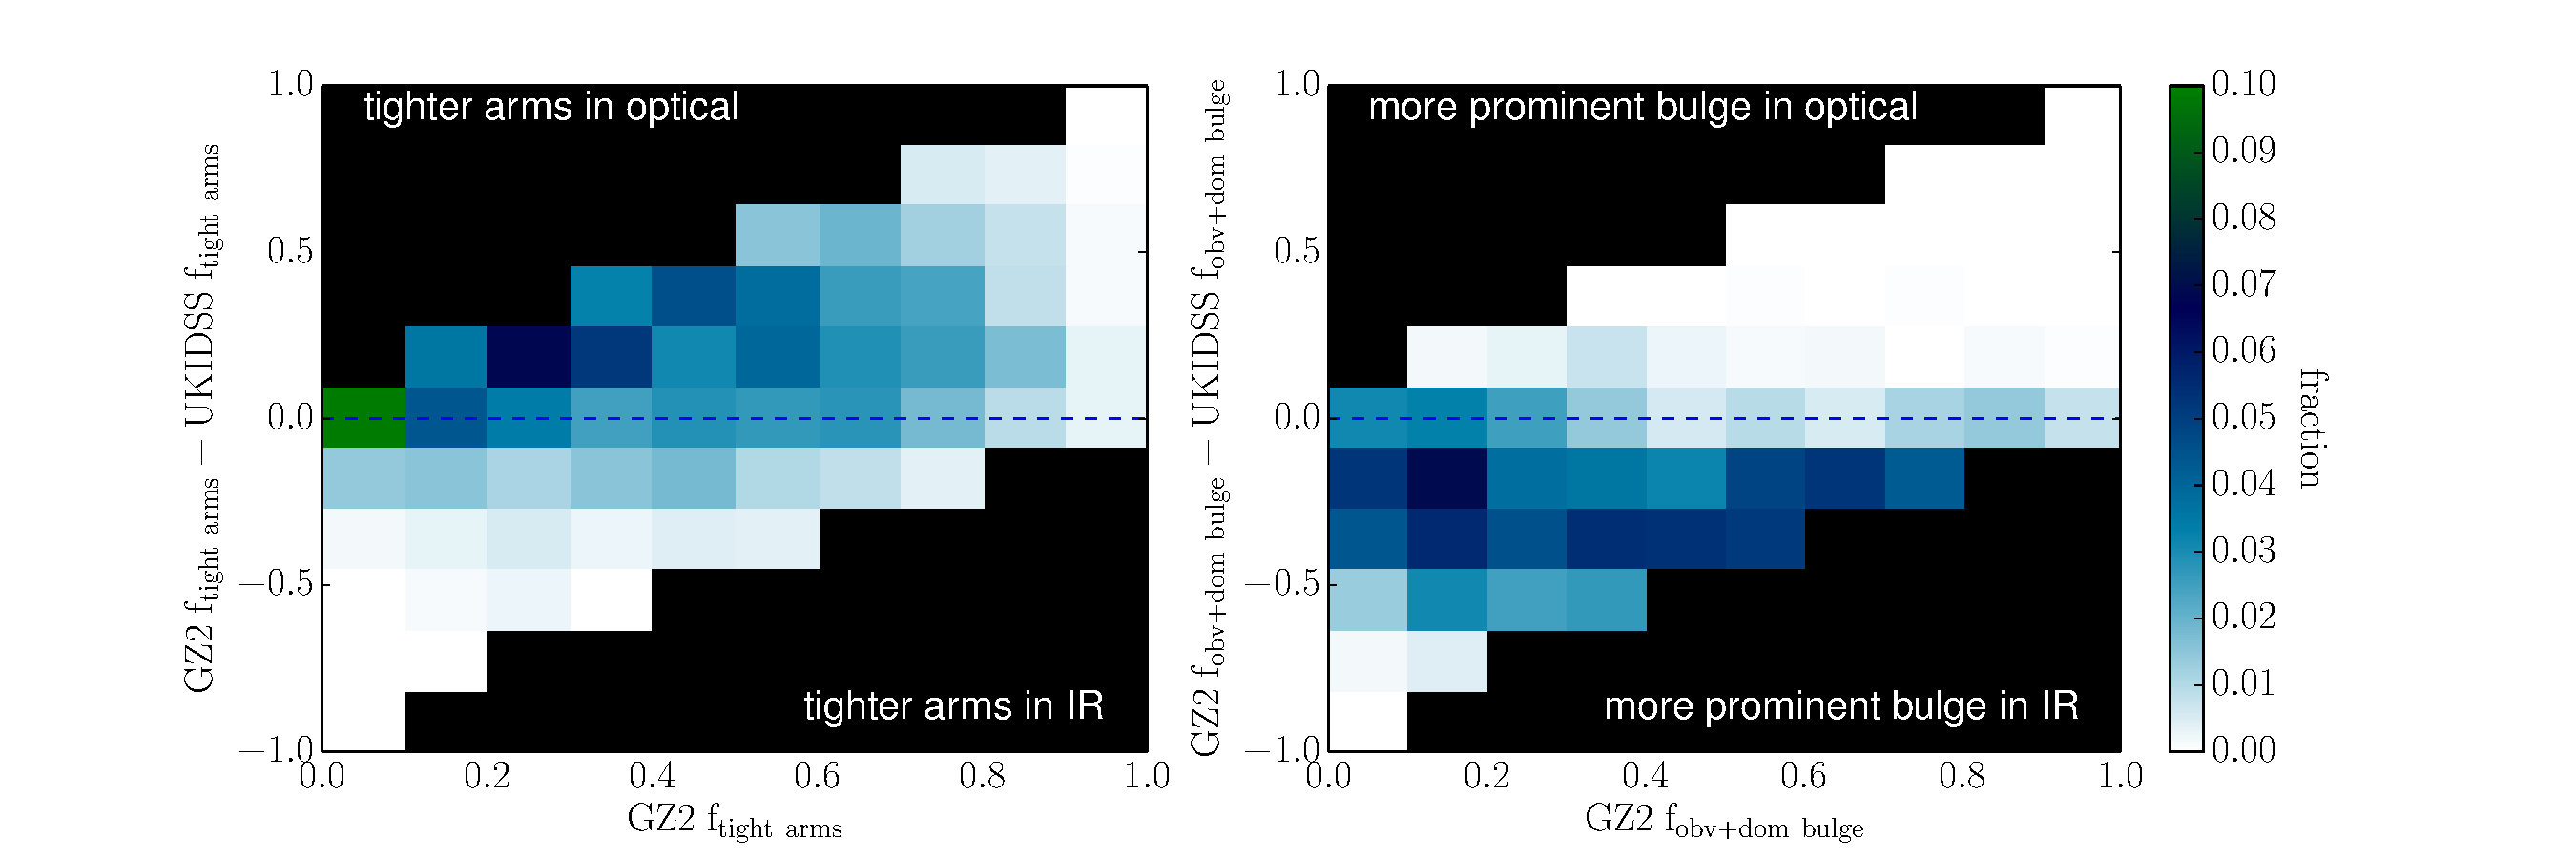
\includegraphics[width=1\textwidth]{figures/t_type.pdf}
\caption{boiiiiii}
\label{fig:ttype}
\end{figure}





 
